\documentclass{standalone}
\usepackage{graphicx}	
\usepackage{amssymb, amsmath}
\usepackage{color}

\usepackage{tikz}
\usetikzlibrary{intersections, backgrounds}
\usepackage{pgfmath}

\definecolor{light}{RGB}{220, 188, 188}
\definecolor{mid}{RGB}{185, 124, 124}
\definecolor{dark}{RGB}{143, 39, 39}
\definecolor{highlight}{RGB}{180, 31, 180}
\definecolor{gray10}{gray}{0.1}
\definecolor{gray20}{gray}{0.2}
\definecolor{gray30}{gray}{0.3}
\definecolor{gray40}{gray}{0.4}
\definecolor{gray60}{gray}{0.6}
\definecolor{gray70}{gray}{0.7}
\definecolor{gray80}{gray}{0.8}
\definecolor{gray90}{gray}{0.9}
\definecolor{gray95}{gray}{0.95}

\begin{document}

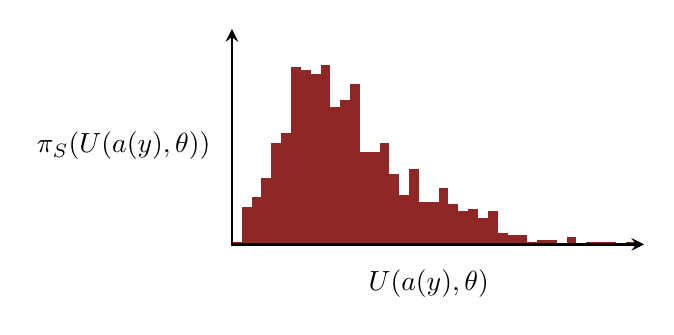
\begin{tikzpicture}[scale=0.5, thick]

  \foreach[count=\n] \y in {0.004, 0.064, 0.080, 0.112, 0.172, 0.188, 0.300, 
                            0.296, 0.288, 0.304, 0.232, 0.244, 0.272, 0.156, 
                            0.156, 0.172, 0.120, 0.084, 0.128, 0.072, 0.072,
                            0.096, 0.068, 0.056, 0.060, 0.044, 0.056, 0.020, 
                            0.016, 0.016, 0.004, 0.008, 0.008, 0.000, 0.012, 
                            0.000, 0.004, 0.004, 0.004, 0.000, 0.004} {
    \fill[dark] ({(\n - 1) / 4}, 0) rectangle ({(\n) / 4}, {15 * \y});
  }

  \node[] at (-2.75, 2.5) { $\pi_{S} (U(a(y), \theta))$ };

  \draw [->, >=stealth, line width=1] (-0.03, 0) -- +(10.5, 0);
  \draw [->, >=stealth, line width=1] (-0, -0.03) -- +(0, 5.5);
  \node[] at (5, -1) { $U(a(y), \theta)$ };

\end{tikzpicture}

\end{document}  